%
% Advanced Robotics submission
% Internal models of reaching and grasping
% Castellini, Orabona, Metta, Sandini
%

\documentclass{arsubmit}
\usepackage{graphicx}
\usepackage{amsmath}
\usepackage[psamsfonts]{amssymb}

\def\RR{\mathbb{R}}
\def\NN{\mathbb{N}}
\def\xx{\mathbf{x}}
\def\ww{\mathbf{w}}
\def\aa{\mathbf{\alpha}}
\def\bb{\mathbf{\beta}}
\def\ee{\mathbf{e}}
\def\dd{\mathbf{d}}
\def\mdd{\tilde{\dd}}
\def\b{\mathcal{B}}
\def\d{\mathcal{D}}

\title{Internal models of reaching and grasping}

\author{Claudio Castellini \and Francesco Orabona \and Giorgio Metta \and Giulio Sandini}

\date{\small \it{
LIRA-Lab and Italian Institute of Technology\\
Genoa, Italy\\
{\tt contact: pasa@liralab.it}
}}

\begin{document}

\maketitle

\begin{abstract}
Grasping is one of the most challenging tasks in advanced robotics...

\end{abstract}

{\it keywords}: human movement, sensing system for daily life,
sensorimotor pattern sand symbol correlation acquisition, motion
capturing systems and its application

\section{INTRODUCTION}
\label{sec:introduction}
It is reasonably well established that the brain stores ``internal
models'' of actions either because they are required to control
movements or, as it has been determined more recently, to interpret
the movements of others \cite{kawato-99, wolpert-03, mussaivaldi-00,
lackner-98}. There is a large body of literature that links the
observation of actions to action execution, like for example the study
of the motor system conducted by Rizzolatti and colleagues in
relatively recent years
\cite{rizzolatti-04,gallese-96,rizzolatti-01}. In the monkey, premotor
area F5 has been particularly well studied and it is in fact the
location where ``mirror neurons'' were first identified. In this
respect, mirror neurons are the quintessential correlate of internal
models since they are activated both when executing a specific
grasping action and when observing a congruent action being executed
by another individual (or the experimenter)
\cite{fadiga-00}.

In a study by Umilt\`a et al. \cite{umilta-01} the response of mirror
neurons to the observation of actions that terminate behind a screen
has been investigated. In this case, the authors analyzed mirror
neurons in situations where the final part of the action was occluded
by an opaque screen with the monkey knowing of the presence/absence of
an object to be grasped. As long as the object was shown to the
monkey, the brain could easily supply the missing visual information
by rehearsing the internal model of the action. The control
experiment, in this case, was that of an identical hand kinematics, an
identical screen but the absence of the target object, that is,
identical visual stimulation apart from the knowledge of the presence
of the object. Elsewhere it has been also shown that the presence of
an object is required to elicit the mirror neurons response in the
monkey \cite{gallese-96}.

{\em A posteriori}, given these results, it is easy to see how the
presence of a target object and its geometrical properties strongly
constrain the type of grasp and the approach to the object, and that,
as a consequence, the brain might need to include this information
when planning an appropriate course of action. In the monkey these
constraints are so strong that mirror neurons do not fire unless the
goal of the action is clearly perceivable. The brain codes for the
object-motor identity in part via another class of F5 visuomotor
neurons called ``canonical neurons'' (for a discussion see for example
\cite{metta-06}). To complete the picture, the work of Graziano,
Hu, and Gross \cite{graziano-97} has shown that the presence of
objects is coded in the ventral premotor cortex and maintained even
when the object is no longer visible as long as there is evidence for
its presence at a particular location.

Relevant to this discussion, the work of Fogassi et
al. \cite{fogassi-05} contributed to the identification of mirror
neurons in the parietal cortex (inferior parietal lobule), which are
thought to be related to the decoding of the intentions of
others. Contextual information which links the enacted action to its
final goal seems to be implicated in this type of neural response. The
presence of objects is a clear contextual cue. In humans, it has been
demonstrated that the activation of brain areas correlated to action
observation is not simply a perceptual effect but rather the
activation of a precise sensorimotor model which includes for example
the hand kinematics \cite{pozzo-06}.
 
Accordingly, Fadiga et al. \cite{fadiga-99,vargas-04} have shown that
motor imagery changes the excitability of the cortico-spinal
connections specifically to the imagined action, that is, imagining a
motor task causes the under-threshold activation of the same neural
pathways required to execute the task. This under-threshold activation
was revealed by transcranial magnetic stimulation. In a conceptually
similar experiment \cite{fadiga-05}, the excitability of
cortico-spinal pathways was also examined as a consequence of the
actual sensory input. In summary, the motor system is similarly
activated when acting in first person, when imagining an action, or
when watching somebody else's action. Jeannerod \cite{jeannerod-88},
for example, goes to a great length in showing how plausible is the
fact that mental imagery uses the same internal models used by actual
action generation.  It is known in this respect that the time required
to simulate an action is the same that is required to execute that
action \cite{sirigu-96}. For a review refer to \cite{jeannerod-99}.

In this paper we set forth to investigate whether a machine equipped
with enough sensory information about human movement could acquire a
similar ``internal model'' via machine learning methods. In
particular, we investigated whether the final configuration of the arm
and hand can be predicted from the initial part of the movement by
imagining that the final part of the action is occluded by a
screen. We analyzed how much error we make in predicting the final
position of the fingers joint angles and the configuration of the
wrist in space: i.e., position and orientation of a coordinate system
fixed with respect to the palm of the hand. We also analyzed whether
the knowledge of the grasped object makes a difference in performance
as it should intuitively do.

In a previous experiment, we analyzed the problem of recognizing hand
gestures visually by incorporating a generative approach that used
motor information explicitly \cite{lopes-05,metta-06}. In that case we
showed that an action recognition system that uses motor information
in a preprocessing step can perform better ($97\%$ recognition rate
versus $80\%$ on the test set) than a traditional classifier built
directly in terms of visual information. This justifies the fact that
as a preprocessing step we can consider a visuo to motor mapping that
transforms the available visual information into motor data. This
procedure is consistent in that it can be trained through 
self-observation. We can imagine that the brain can exercise its
control and simultaneously acquire both the motor commands and the
corresponding visual information and learn such a mapping. In the
following, we will only consider motor information since we can safely
assume that the visuo-motor map can always incorporated in the global
internal model.

If actually realised, such internal models could potentially be used
in various ways including the control of semi-autonomous teleoperated
/ prosthetic robotic artifacts, the interpretation of human movements,
and clearly they can be used to reproduce and mimic human movements
\cite{wolpert-01}. For example, in controlling or teleoperating an
anthropomorphic robotic platform, we can guess the user intention and
ask the robot to complete the action autonomously. Predicting the user
intention finds its natural role in building man-machine interfaces
and possibly into the control of prosthetic devices.

The paper is structured as follows: we describe the methods and the
experimental setup in section \ref{sec:exp_desc} and the results
obtained in section \ref{sec:exp_res}; lastly we discuss them and
comment on future development in section \ref{sec:Conclusions}.


\section{SUPPORT VECTOR MACHINES}
\label{sec:svm}
Assume $\{\xx_i,y_i\}_{i=1}^l$, with $\xx_i \in \RR^m$ and $y_i \in
\{-1,1\}$, is a set of samples drawn from an unknown probability
distribution. The problem is to approximate it in order to classify
more data coming from the same source to the best extent
possible. Assuming the data are linearly separable, according to the
standard approach, a \emph{separating hyperplane} in $\RR^m$ is sought
for:

\begin{equation} \label{eqn:dec}
  f(\xx) = sgn(\ww\cdot\xx + b)
\end{equation}

\noindent with $\ww \in \RR^m$ and $b \in \RR$. In this case, the
hyperplane must respect the constraints $y_i(\ww\cdot\xx_i + b)-1\geq
0$, for all $i = 1,\ldots,l$ (from now on, this will be implicit
whenever a subscript $i$ appears free in a formula). In the general,
more likely and realistic case in which the data are not linearly
separable, we introduce $l$ slack variables $\xi_i$ and rather require
that $y_i(\ww\cdot\xx_i + b)-1+\xi_i\geq 0$, with $\xi_i \geq 0$. In
order to find such a hyperplane, we wish to maximise the hyperplane's
distance from both groups of samples (\emph{margin}). The margin is
easily determined to be $\frac{2}{||\ww||}$, so we are left with the
problem of minimising $||\ww||$ subject to the above constraints. The
problem is then usually solved minimising the following expression:

\begin{equation} \label{eqn:svm_primal}
  \min_{\ww} \left( ||\ww||^2 + C \sum_{i=1}^l \xi_i \right)
\end{equation}

\noindent subject to the constraints

\begin{eqnarray} \label{eqn:svm_constr}
  y_i (\ww\cdot\xx_i + b) & \geq & 1-\xi_i \\
                    \xi_i & \geq & 0 \nonumber
\end{eqnarray}

\noindent where $C \in \RR$ is a positive weight coefficient. Since
both the problem and the constraints are convex,
(\ref{eqn:svm_primal}) and (\ref{eqn:svm_constr}) can be compactly
expressed in Lagrangian form by introducing $l$ pairs of coefficients
$\alpha_i, \mu_i$ and then minimising the objective function

\begin{equation} \label{eqn:lp1}
  L_P =
      \frac{1}{2} ||\ww||^2
    - \sum_{i=1}^l \alpha_i \left(y_i (\ww\cdot\xx_i+b) - 1 + \xi_i \right)
    + C \sum_{i=1}^l \xi_i
    - \sum_{i=1}^l \mu_i \xi_i
\end{equation}

\noindent subject to the constraints that $\alpha_i,\mu_i\geq 0$. By
using the extremum conditions for $\ww$ and $b$, that is,
$\nabla_{\ww,b} L_P = 0$, one finds that

\begin{equation} \label{eqn:w1}
  \ww = \sum_{i=1}^l \alpha_i y_i \xx_i
\end{equation}

\noindent which, substituted in Equation (\ref{eqn:dec}), gives

\begin{equation} \label{eqn:lin_sol}
  f(\xx) = sgn \left( \sum_{i=1}^l \alpha_i y_i \xx \cdot \xx_i + b \right)
\end{equation}

Notice that, in the last Equation, the $\xx$'s only appear in the form
of inner products; in order to boost the expressive power of SVMs
then, the $\xx_i$s are usually mapped to a highly, possibly
infinite-dimensional space (the \emph{feature space}) via a
non-linear mapping $\Phi(\xx)$; the core of the SVM becomes then the
so-called \emph{kernel function} $K$ such that $K(\xx_1,\xx_2) =
\Phi(\xx_1)\cdot\Phi(\xx_2)$. This idea is called \emph{kernel trick}
and is standard in literature; it avoids the necessity of explicitly
knowing $\Phi$. Equation (\ref{eqn:lin_sol}) then becomes

\begin{equation} \label{eqn:sol}
  f(\xx) = sgn \left( \sum_{i=1}^l \alpha_i y_i K(\xx,\xx_i) + b \right)
\end{equation}

After training, that is after the minimisation of $L_P$, some of the
$\alpha_i$s (actually most of them in many practical applications) are
zero; those $\xx_i$s for which this does \emph{not} hold are somehow
crucial to the solution and are called \emph{support vectors}, hence
the name of the approach. This phenomenon is known as
\emph{sparseness} of the solution, meaning that only a subset of the
training data is usually really needed to build it.


\section{MATERIALS AND METHODS}
\label{sec:exp_desc}
\subsection*{Devices}

We collected data using a 22-sensors Immersion DataGlove for the hand
posture, an Ascension Flock-Of-Birds (FoB) for the hand position and a
Force Resistor Sensor (FSR) to detect the contact moment with the
object.

The DataGlove was worn by the subject on the right hand. The device
returns $22$ $8$-bit numbers, describing the position of the three
phalanxes of each finger (for the thumb, rotation and two phalanxes),
the four finger-to-finger abductions, the palm arch, the wrist pitch
and the wrist yaw. The FoB sensor was firmly mounted on the DataGlove,
just above the subject's wrist, with the X/Y plane being parallel to
the palm plane in the resting position. The device returns $6$
double-precision numbers describing the position ($x$, $y$ and $z$ in
inches) and rotation (azimuth, elevation and roll in angles) of the
sensor with respect to a magnetic basis mounted about one meter away
from the subject. The FSR was mounted on the subject's thumb. It
returns a $32$-bit number approximately inversely proportional to the
pressure applied to the surface of the sensor. All devices were tuned
to stream at $100$Hz, and their data were synchronised, collected and
saved in real time. Figure \ref{fig:devices} shows the devices, as
worn by a subject.

\begin{figure}[htbp]
  \begin{center}
    \begin{tabular}{cc}
      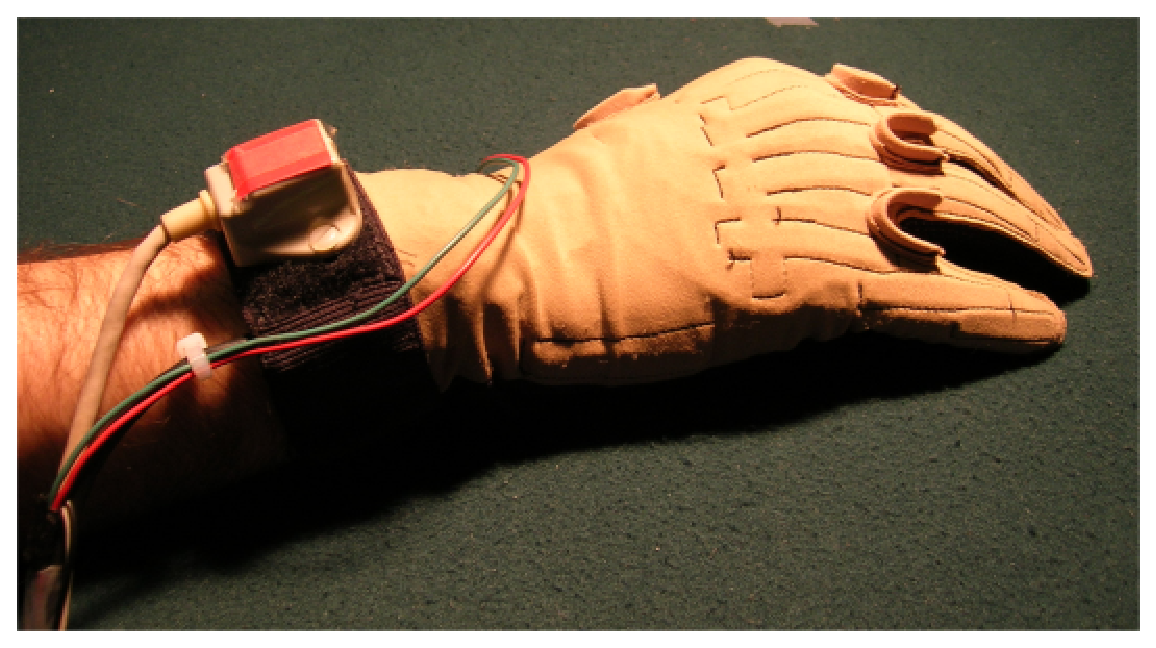
\includegraphics[width=0.45\linewidth]{devices1.eps} &
      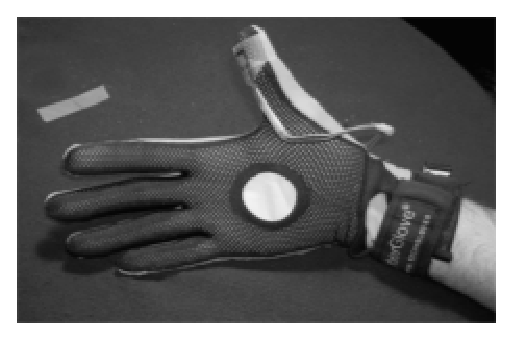
\includegraphics[width=0.45\linewidth]{devices2.eps} \\
      $(a)$ & $(b)$
    \end{tabular}
    \caption{The devices used for the experiment, as worn by a
    subject: $(a)$ the DataGlove with the Flock-of-Birds just above the
    subject's wrist; $(b)$ the Force Resistor Sensor attached to the
    subject's thumb.}
    \label{fig:devices}
  \end{center}
\end{figure}

\subsection*{Subjects}

Eleven subjects, four females and seven males aged $24$ to $34$ of
several different nationalities, joined the experiment. They were all
right-handed and fully able-bodied, and were given initially some
knowledge of the aim of the experiment.

\subsection*{Experimental setup}

The subjects were asked to sit confortably in front of a clean
workspace of about one squared meter, at the center of which an object
was placed, in a predefined position. The subjects were then asked to
wear the DataGlove (along with the FoB and FSR), and to choose a
resting position for their right hand and arm.

The subjects had to grasp the object with their right hand any way
they wanted, not necessarily the same way each time, keeping a
``natural'' attitude, i.e., without employing weird hand positions
and/or postures, but being able to seize the object with precision or
power grips, using the whole hand cilyndrically or just a subset of
their fingers, etc. After grasping the object, they had to drop it
somewhere else in the workspace, and then return their right hand and
arm in the initial resting position. Subsequently, they had to use
their left hand to reposition the object roughly in the same place it
was before.

We first had the subjects do a trial run of the experiment, in order
for them to gain confidence in the setup. A beeping sound was heard
each time the subject made contact with the object (that is, each time
the FSR signalled a significant change), and they were asked to try
and hear the beep each time they grasped the object. Although this
ruled out grasps which made no use of the thumb, it enabled us to
better understand the contact point.

After the trial run, subjects were asked to repeat the
grasp/drop/reposition procedure $120$ times per each object. We
employed, in turn, three objects: a beer can, a scotch tape roll and a
mug (Figure \ref{fig:objects} shows the objects).

\begin{figure}[htbp]
  \begin{center}
    \begin{tabular}{ccc}
      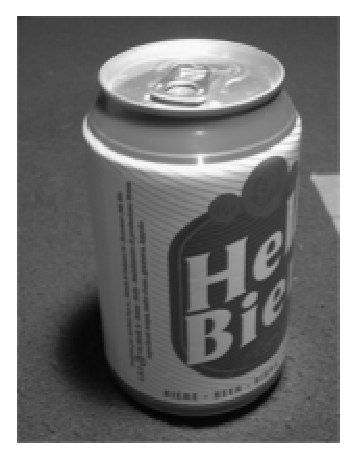
\includegraphics[width=0.3\linewidth]{beer.eps} &
      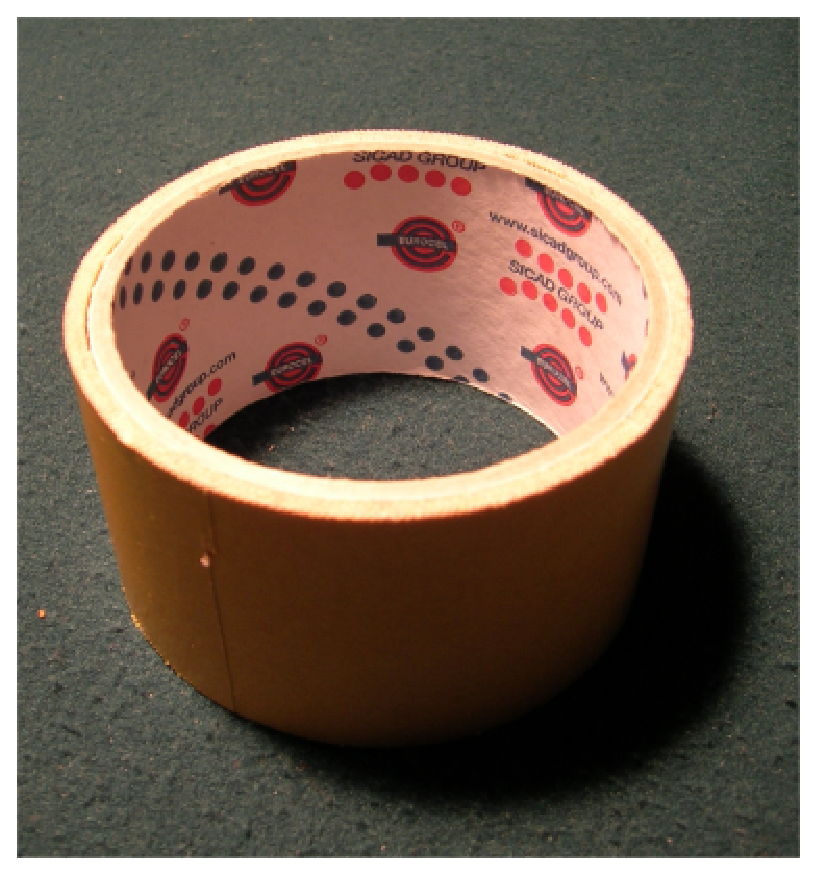
\includegraphics[width=0.3\linewidth]{scotch.eps}  &
      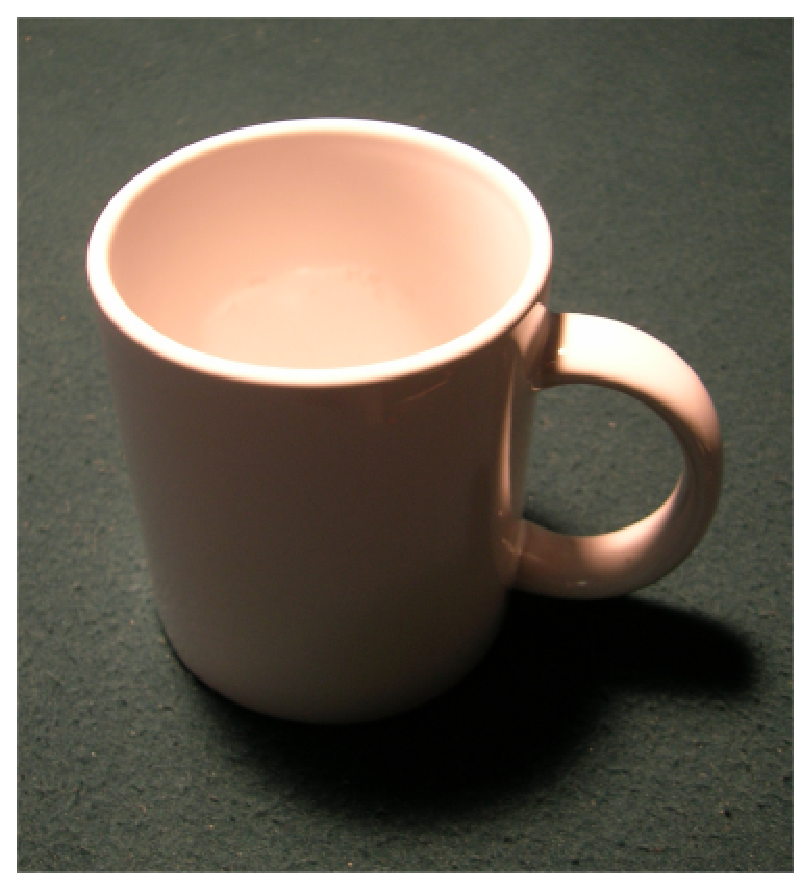
\includegraphics[width=0.3\linewidth]{mug.eps} \\
      $(a)$ & $(b)$ & $(c)$
    \end{tabular}
    \caption{The objects used inthe experiment: a beer can $(a)$, a scotch
    tape roll $(b)$ and a mug $(c)$.}
    \label{fig:objects}
  \end{center}
\end{figure}

The $120$-grasps session was done twice, resulting in approximately
$240$ grasps for each of the three objects. In order not to have the
subjects ``specialise'' on a particular object, we alternated the
sessions this way: first the can, then the roll and then the mug, all
of this two times.

Experiments lasted $35$ to $56$ minutes depending on the subject's
confidence and speed; although almost no subjects reported tiredness,
we allowed for rest between each session. It was reported by almost
every subject that the experiment became rapidly boring, which lets us
claim that almost all grasps were done in a natural, almost
unconscious way. Figure \ref{fig:setup} shows the main phases of the
experiment.

\begin{figure}[htbp]
  \begin{center}
    \begin{tabular}{ccc}
      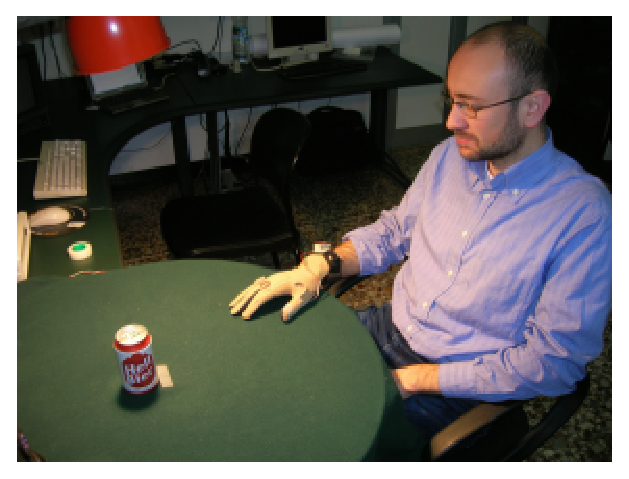
\includegraphics[width=0.3\linewidth]{exp1.eps} &
      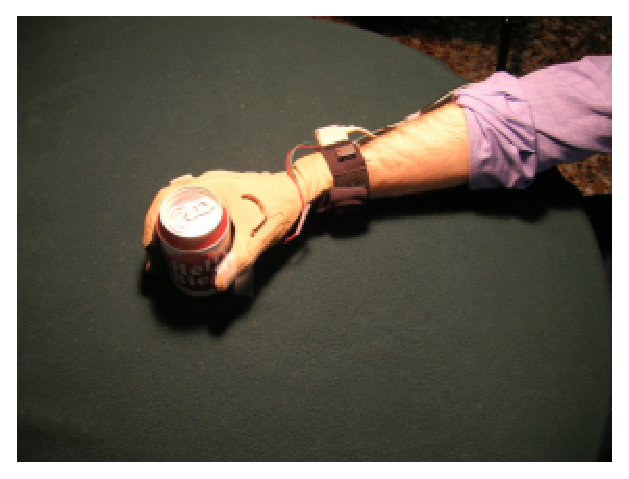
\includegraphics[width=0.3\linewidth]{exp2.eps}  &
      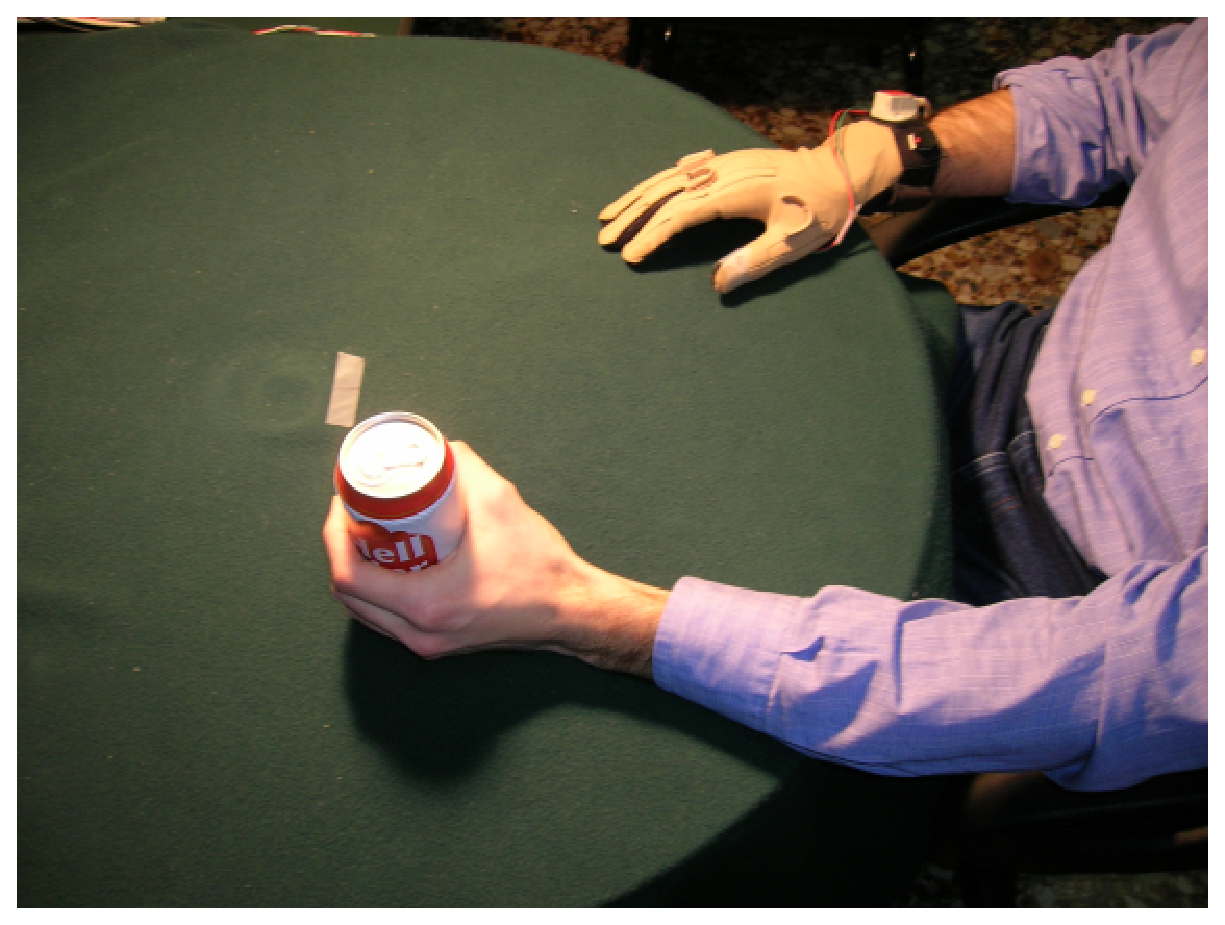
\includegraphics[width=0.3\linewidth]{exp3.eps} \\
      $(a)$ & $(b)$ & $(c)$
    \end{tabular}
    \caption{The experiment. The subject sits confortably in
    front of a clean workspace, at the center of which an object is
    placed $(a)$, with his right hand in a resting position. He then
    grasps the object and drops it somewhere else in the workspace
    $(b)$, bringing then his arm and hand in the resting
    position. Lastly, he repositions the object in the initial
    position using his left arm and hand $(c)$. The procedure is repeated
    for $120$ times, then this session is repeated for each of the
    three objects, and all of this is done twice, resulting in
    approximately $240$ grasps for each subject and object.}
    \label{fig:setup}
  \end{center}
\end{figure}

\subsection*{Data Analysis and Pre-processing}


\section{RESULTS}
\label{sec:exp_res}
% anno del balasko
% due citazioni sul clustering
% visualizzare posture e mettere le figure

We were mainly interested in answering two questions:

\begin{enumerate}

  \item how far in the future can our system predict well?

  \item how does the knowledge of the grasped object affect the error?

\end{enumerate}

In order to answer the first question, we have checked how the error
on regression changes as $B$ varies from $0.1$ to $0.5$. This
procedure was repeated independently for each single sensor.

To obtain statistically meaningful results, we recorded each mean
error obtained \emph{on a single fold} of the cross-validation
procedure; for each sensor and value of $B$, this means we have
obtained $5$ numbers. The errors for each sensor were then grouped
accordingly to their measurement units and meaning: the position of
the hand ($3$ sensors, the $x,y,z$ from the FoB), the hand orientation
($3$ sensors, the azimuth, elevation and roll from the FoB), and the
posture of the hand ($22$ sensors, the joint positions from the
CyberGlove). According to the device resolutions (see the previous
Section), we set $\epsilon$ to $0.1$ inches for the hand position,
$0.5$ degrees for the hand orientation and $1$ degree for the hand
posture.

Lastly, for each group of sensors, we averaged the errors \emph{per
single cross-validaton fold}, and evaluated the mean and standard
deviation of these $5$ values. This gave us an indication of how well
our machine performed on the hand position, orientation and posture. In
all graphs, the points on the curves represent the mean values,
whereas the error bars are placed at $\pm 1$ standard deviations.

In order to answer the second question, we first evaluated the error
obtained as described above using all sessions for each single object,
so to obtain an estimate of how complex it is to approximate the grasp
for the can, roll and mug unbiased by the differences among the
subjects. Subsequently we averaged these three errors and compared the
averages with the overall error, obtained by joining \emph{all}
sessions together in a single training set.

\subsection{Prediction power}

Figure \ref{fig:err_all} shows the main experimental results.

\begin{figure}[htbp]
  \begin{center}
    \begin{tabular}{cc}
      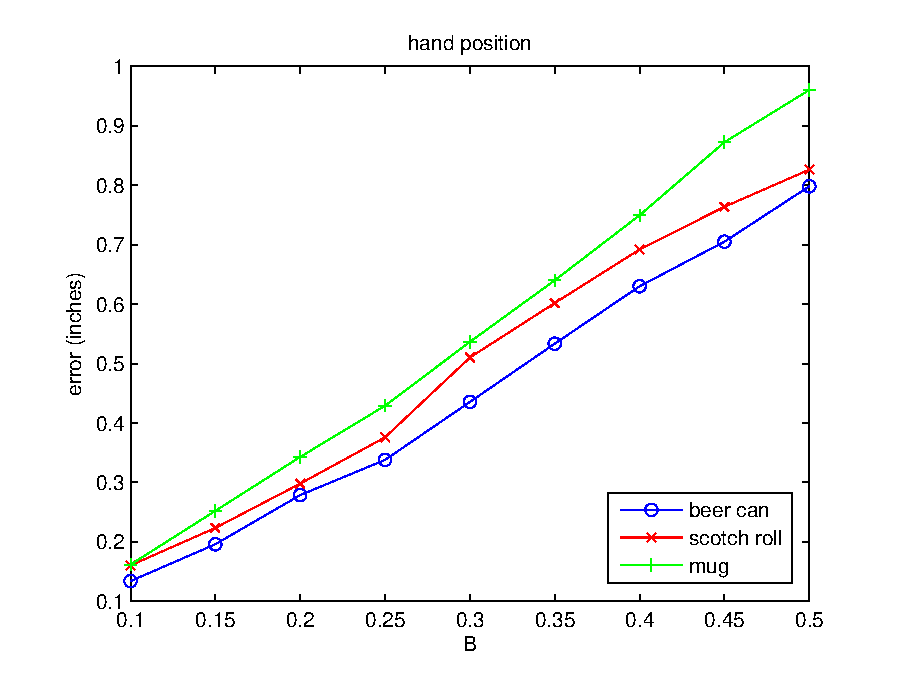
\includegraphics[width=0.45\textwidth]{error_pos.eps} &
      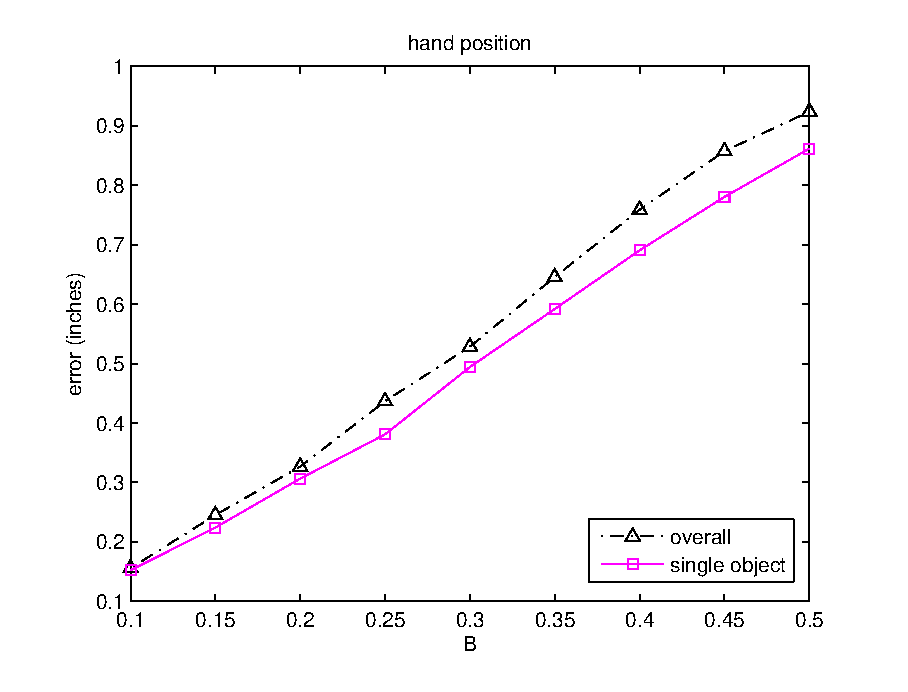
\includegraphics[width=0.45\textwidth]{error_cmp_pos.eps} \\
      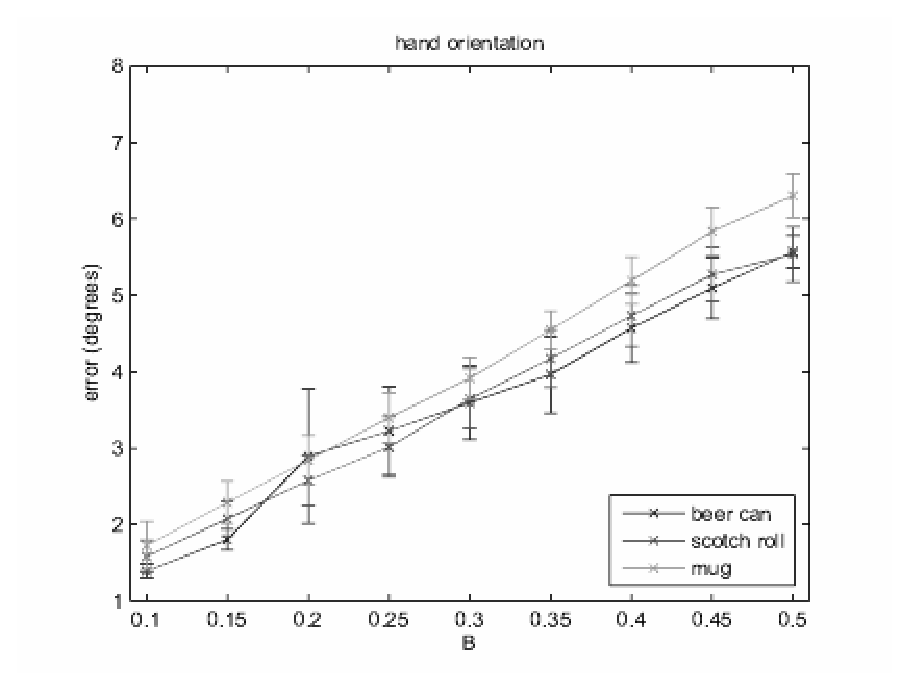
\includegraphics[width=0.45\textwidth]{error_ori.eps} &
      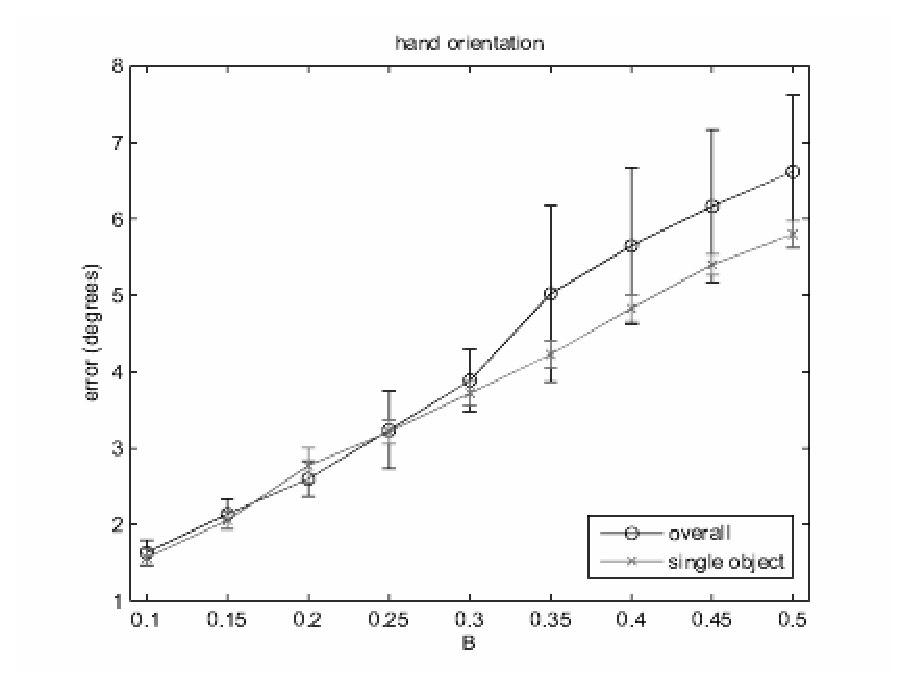
\includegraphics[width=0.45\textwidth]{error_cmp_ori.eps} \\
      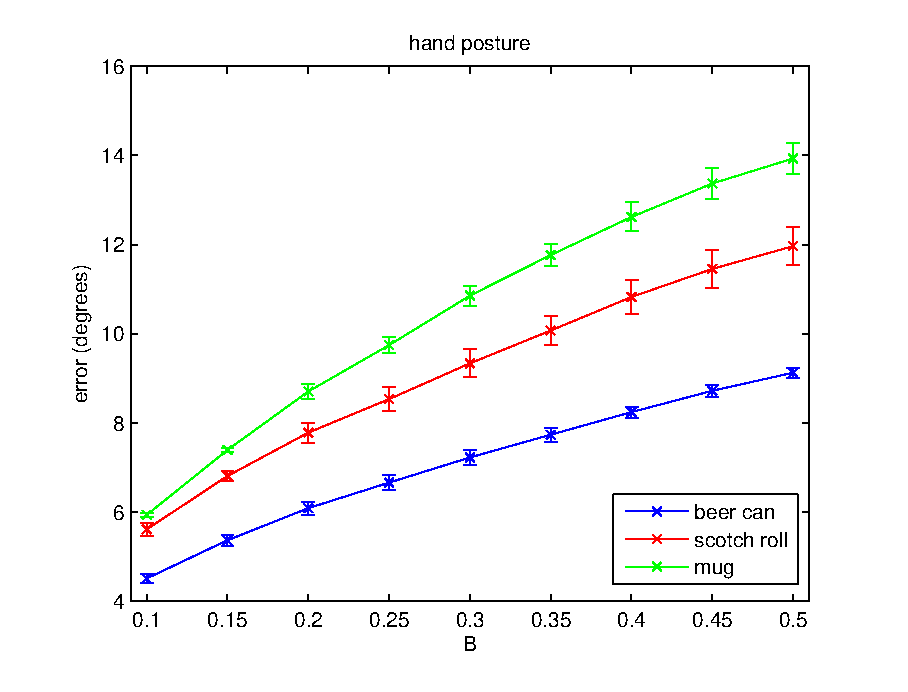
\includegraphics[width=0.45\textwidth]{error_pst.eps} &
      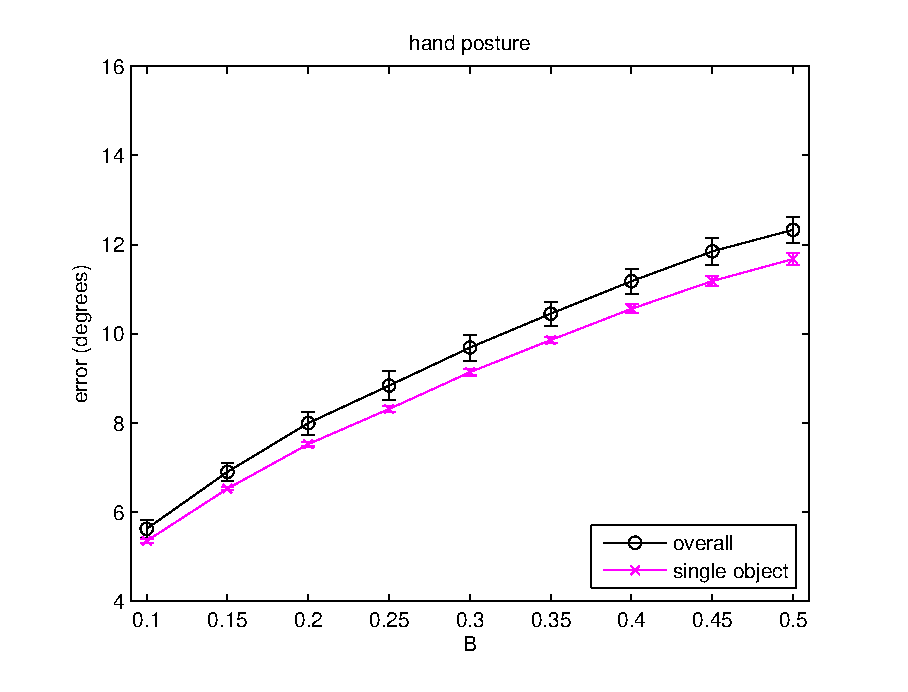
\includegraphics[width=0.45\textwidth]{error_cmp_pst.eps} \\
    \end{tabular}
    \caption{Regression results as the blind fraction $B$ increases
    from $0.1$ to $0.5$. In each row the
    left-hand side pictures compare the errors on different objects,
    while the right-hand side pictures compare the average error on
    single objects and the overall error.}
    \label{fig:err_all}
  \end{center}
\end{figure}

Consider Figure \ref{fig:err_all}, left column: first of all, as $B$
increases, the error does, as it was intuitively expected: the more
data is hidden, the harder the prediction becomes. Then, as one can
see, as far as the hand position and orientation are concerned, the
three objects show comparable errors. On the other hand, there is a
precise ranking in the hand posture regression: the mug is more
difficult than the scotch roll, which is in turn harder than the beer
can. This also is intuitively sensible, since it is possible to grasp
the scotch roll in more ways than the can, and it is possible to grasp
the mug in even more ways (especially, using the handle).

A further analysis of the obtained models (see Figure
\ref{fig:hyperp}, left column) shows that, accordingly, the percentage
of Support Vectors with respect to the total number of samples
increases steadily as $B$ grows, indicating that the problem becomes
harder and harder. The three curves also confirm that regression on
the mug is the most difficult, followed in turn by the scotch roll and
the beer can.

\begin{figure}[htbp]
  \begin{center}
    \begin{tabular}{cc}
      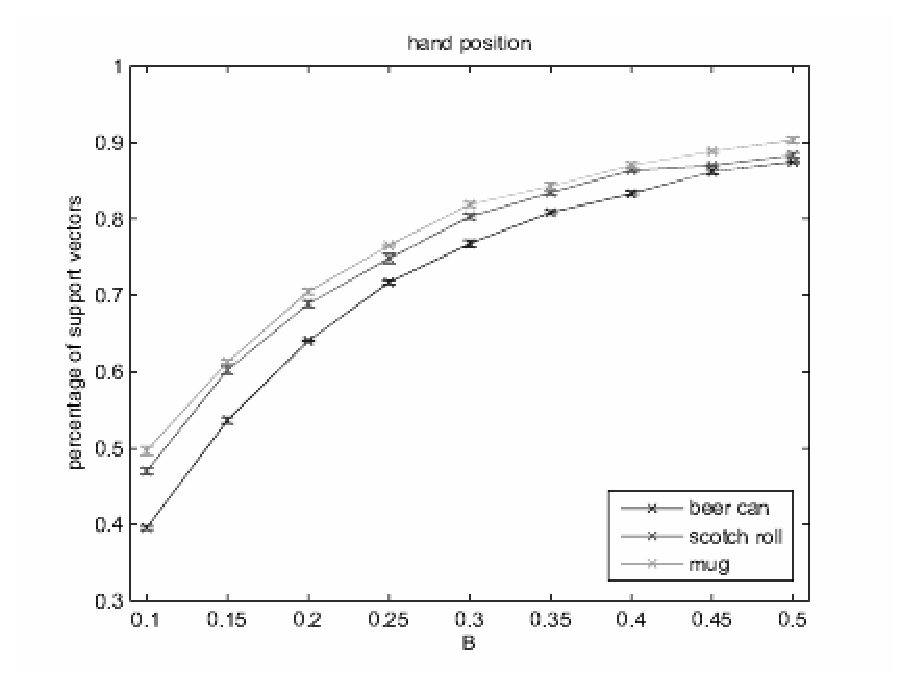
\includegraphics[width=0.45\textwidth]{error_pos_SV.eps} &
      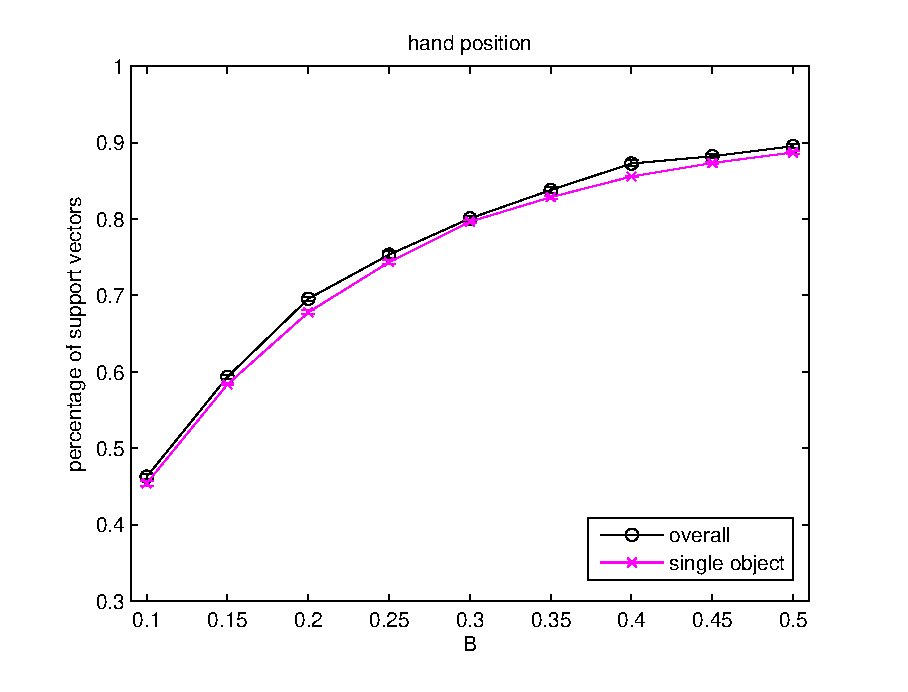
\includegraphics[width=0.45\textwidth]{error_cmp_pos_SV.eps} \\
      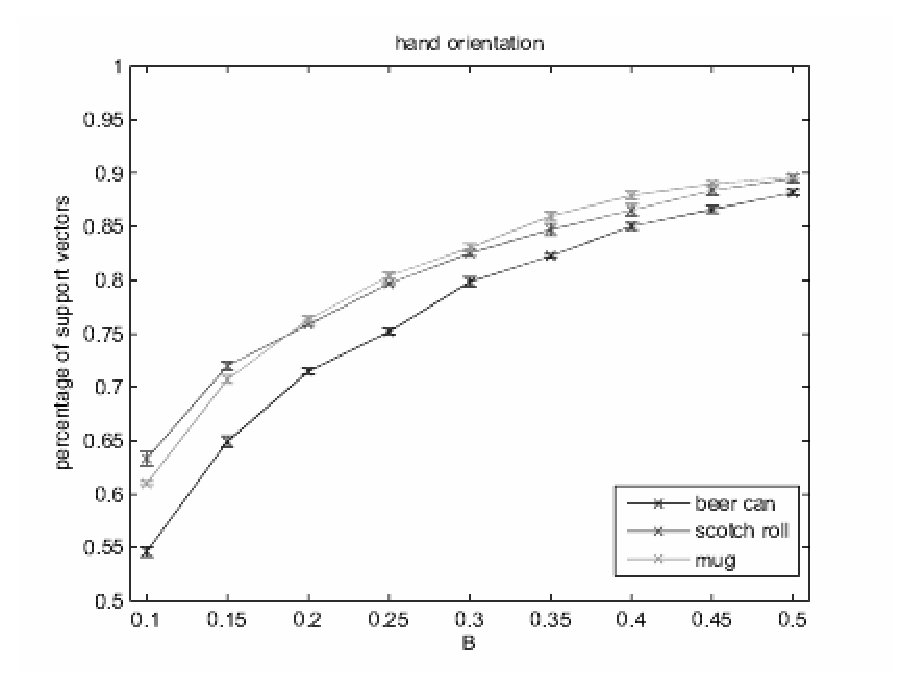
\includegraphics[width=0.45\textwidth]{error_ori_SV.eps} &
      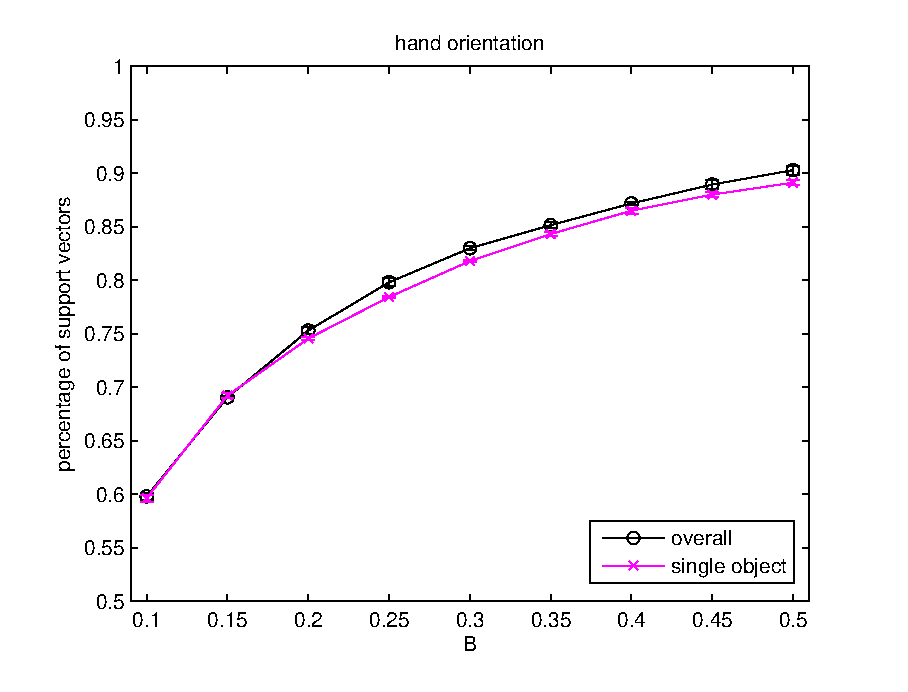
\includegraphics[width=0.45\textwidth]{error_cmp_ori_SV.eps} \\
      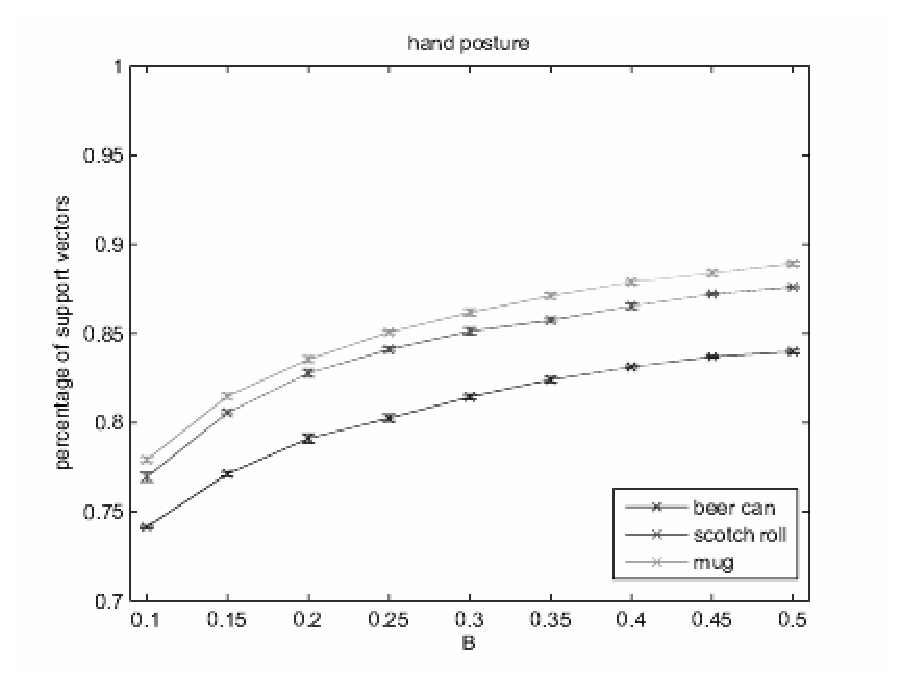
\includegraphics[width=0.45\textwidth]{error_pst_SV.eps} &
      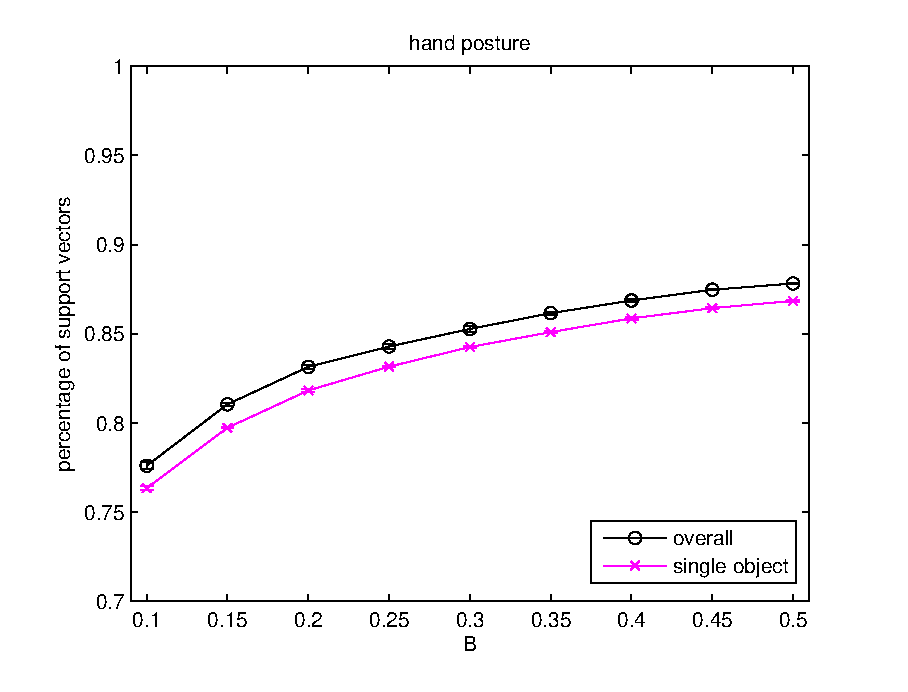
\includegraphics[width=0.45\textwidth]{error_cmp_pst_SV.eps} \\
    \end{tabular}
    \caption{Percentage of support vectors with respect to the total
    number of samples.}
    \label{fig:hyperp}
  \end{center}
\end{figure}

A further analysis of the hyperparameters (see Figure
\ref{fig:C_trend}) confirms that, as $B$ increases, more and more
information is missing from the training set: both $C$ and $\sigma$
show a decreasing trend on all three groups of sensors (more
pronounced in the case of $C$), meaning that the regularisation term
in Equation (\ref{eqn:svm_primal}) becomes more and more important.

\begin{figure}[htbp]
  \begin{center}
    \begin{tabular}{cc}
      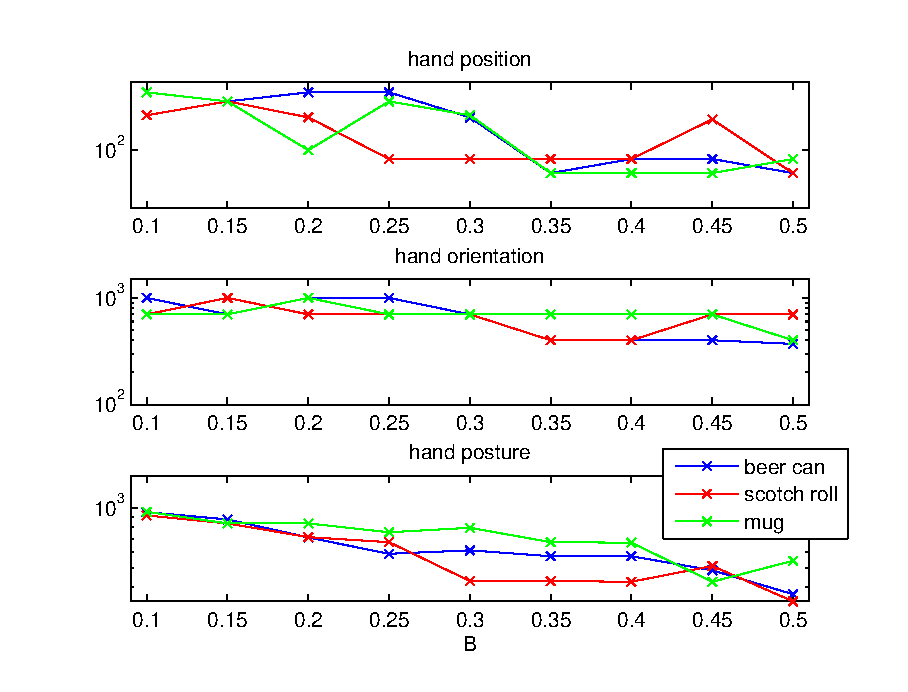
\includegraphics[width=0.45\linewidth]{trend_C.eps} &
      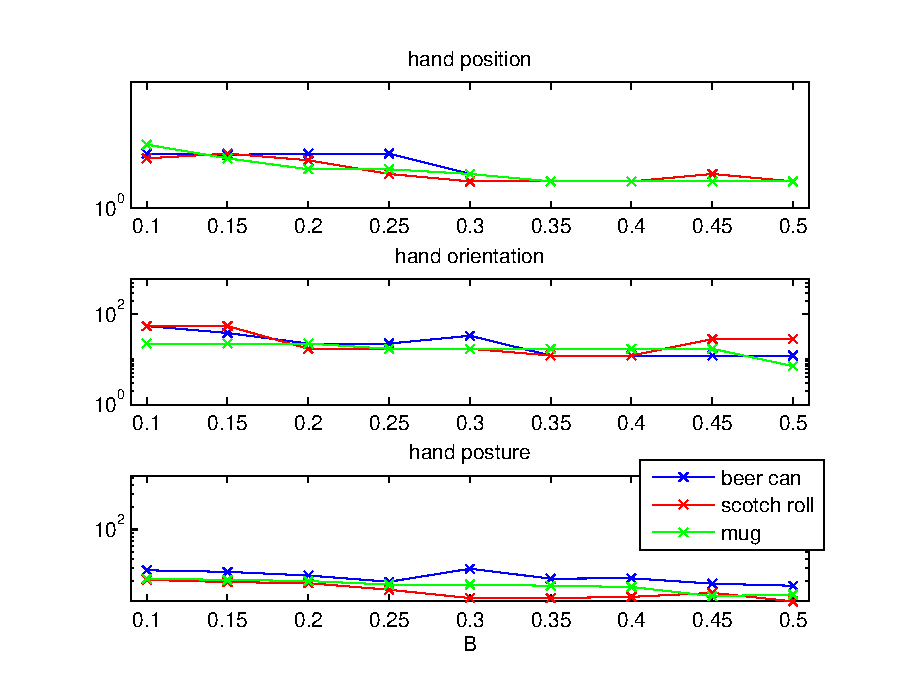
\includegraphics[width=0.45\linewidth]{trend_sigma.eps}
    \end{tabular}
    \caption{The trend of the hyperparameters $C$ (left pane) and
    $\sigma$ (right pane), as far as the hand position, orientation
    and posture is concerned. As $B$ is increased, both parameters show a
    decreasing trend, more pronounced in the case of $C$.}
    \label{fig:C_trend}
  \end{center}
\end{figure}

To determine how far in the future SVMs can predict well, we need to
decide what an acceptable error is. In general, this is
application-dependent. In this case we decided to accept an error as
large as $5$ times a minimum threshold, determined by taking into
account the resolutions of the sensors as declared in the devices
manuals and related publications (see the previous Section). This lead
us to $0.5$ inches for the hand position, $2.5$ degrees for the hand
orientation, and $7.5$ degrees for the hand posture. As far as the
hand posture is concerned, it must be remarked that, in this paper, we
have only considered the average of errors on all the $22$ sensors,
whereas in a more detailed analysis one should take into account that,
e.g., an error on the wrist pitch would lead to a worse displacement
of the hand, than an error on a phalanx would. This is subject of
future research.

As one can see from the graphs, the acceptable error is attained for
the hand position at $B=0.3$, for the hand orientation at $B=0.2$ and
for the hand posture at $B=0.15$ (mug), $0.2$ (scotch roll) and
$B=0.35$ (beer can). Since the average grasp lasts on average $0.62$
seconds, we can say that the system can predict reasonably well

\begin{itemize}

  \item something less than $200$ milliseconds in advance the hand
    position,

  \item about $120$ milliseconds in advance the hand orientation, and

  \item about $100-200$ milliseconds in advance the hand posture, the
    mug being the hardest and the beer can the easiest object.

\end{itemize}

This answers the first question.

\subsection{Knowledge of the objects}

As far as the second question is concerned, consider Figure
\ref{fig:err_all}, right column: the curve representing the error on
the single objects is basically always smaller than the other one,
indicating that a specific SVM trained on a single object will on
average be more precise than a SVM trained on all objects altogether:
the \emph{a priori} knowledge of the object improves the
performance.

Notice that this effect is more pronounced in the case of the hand
posture than for the hand position and orientation, where a
substantial overlap of the error bars can be seen (the ANOVA test on
the time series indicates low significance for the hand position and
orientation, but high significance for the posture). This is sensible,
since knowing \emph{what object} one is going to grasp will tell a
great deal about \emph{how to shape one's hand} in order to grasp it,
but it will definitely be less influential in order to determine where
and how to \emph{reach}.

Let us now focus upon the fraction of SVs found by the SVMs: consider
Figure \ref{fig:hyperp}, right column, again. It turns out that SVMs
trained on single objects have a \emph{definitely smaller} fraction of
SVs than the one trained on the overall sequence. This means that the
machines trained on single objects \emph{are smaller and simpler than
the overall one, while being more precise.}

Summing up, we can say that if the problem is split into subproblems,
each one regarding a single object, performances are better and the
computational complexity is smaller. This phenomenon is particularly
evident as far as the hand posture is concerned, as one can
intuitively expect.

This answers the second question.

\subsection{Single grasp types}

A further interesting question is:

\begin{itemize}

  \item how well does our system perform on \emph{specific types of
    grasp}?

\end{itemize}

In order to shed light on this point, we have considered the most
complex and interesting object under this point of view, i.e., the
mug. All sessions in which the subjects were grasping the mug have
been collected, and all final grasping hand postures have been
considered as representing the ways the mug was grasped. This resulted
in slightly more than $2550$ samples, according to the fact that each
of the $11$ subjects performed about $240$ mug grasps.

The final positions were then clustered using a K-means clustering
algorithm (see, e.g., \cite{...}). We used the freely available
\emph{Fuzzy Clustering and Data Analysis Toolbox}) Matlab toolbox
\cite{fctBalasko}; due to the intrinsically stochastic nature of the
algorithm, we ran the algorithm $100$ times for $1,\ldots,10$ clusters
and employed Dunn's Index \cite{...} to determine what was the optimal
number of clusters. It was determined that the optimal number of
clusters was $4$, corresponding to the four hand postures visible in
Figure \ref{fig:postures}.

\begin{figure}[htbp]
  \begin{center}
    \begin{tabular}{cccc}
      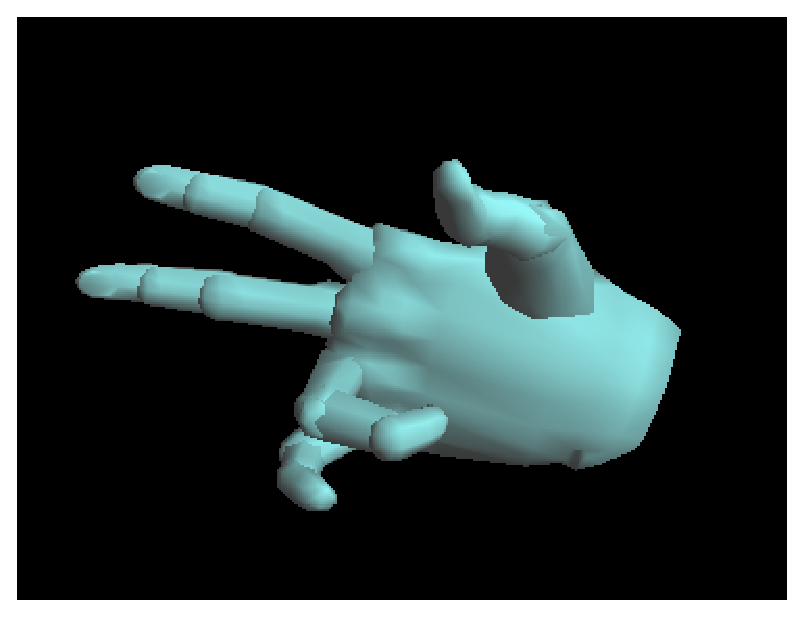
\includegraphics[width=0.22\linewidth]{posture1.eps} &
      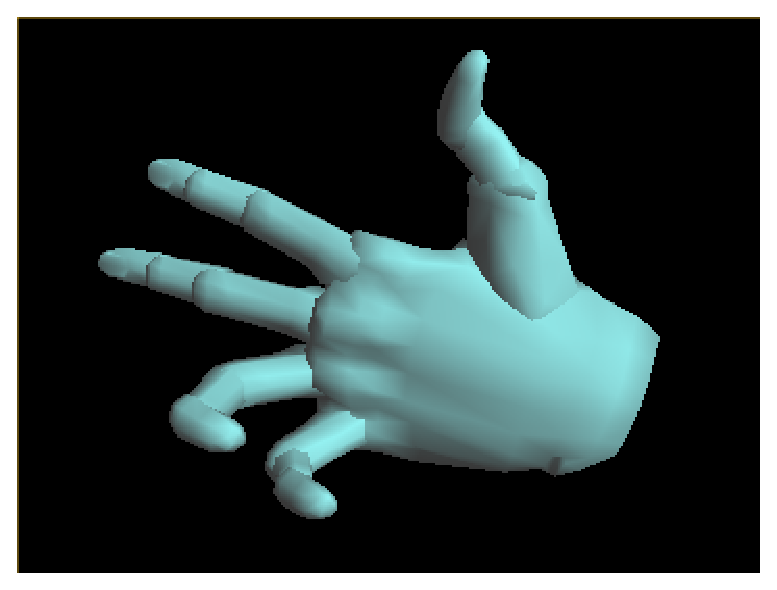
\includegraphics[width=0.22\linewidth]{posture2.eps} &
      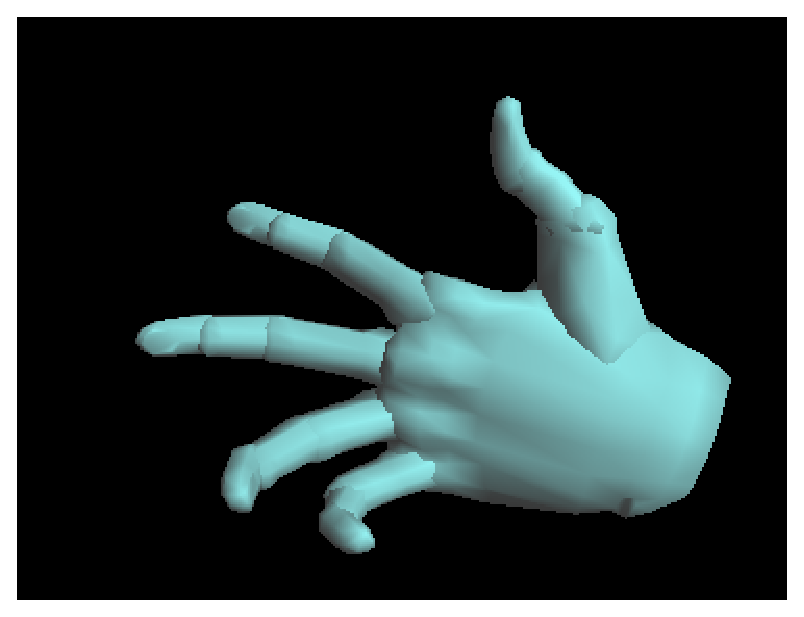
\includegraphics[width=0.22\linewidth]{posture3.eps} &
      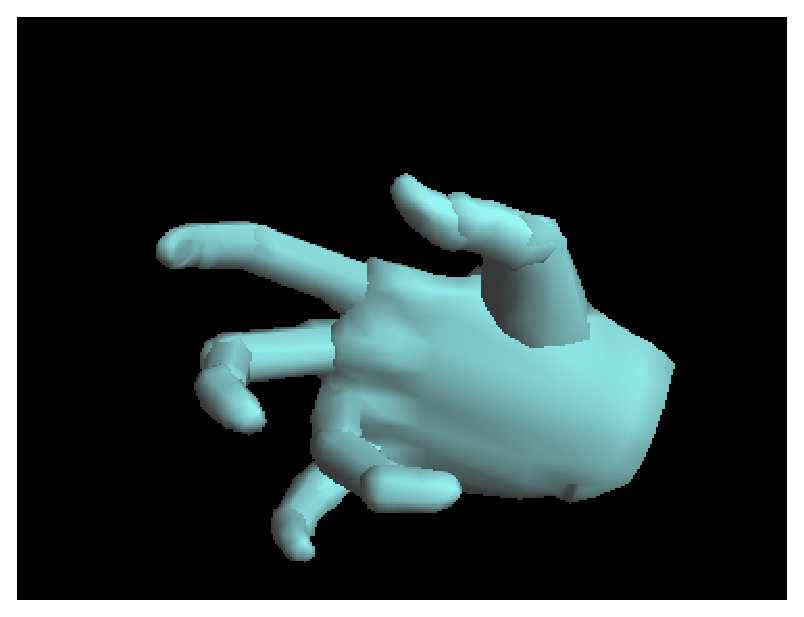
\includegraphics[width=0.22\linewidth]{posture4.eps} \\
      (1) & (2) & (3) & (4) \\
    \end{tabular}
    \caption{The four prototypical hand postures when grasping the
      mug, as found by K-means clustering.}
    \label{fig:postures}
  \end{center}
\end{figure}

We then split the mug grasps into four sets according to the
clustering, and ran separate experiments on each set for
$B=0.1,\ldots,0.5$; lastly, we compared the four error and SV
percentage curves to one another, and to the mug curve of Figures
\ref{fig:err_all} and \ref{fig:hyperp}, left column, bottom graph. We
hoped to get more insight on how the knowledge of what grasp is being
examined changed the situation. Figure \ref{fig:clustering} shows the
experimental results.

\begin{figure}[htbp]
  \begin{center}
    \begin{tabular}{cc}
      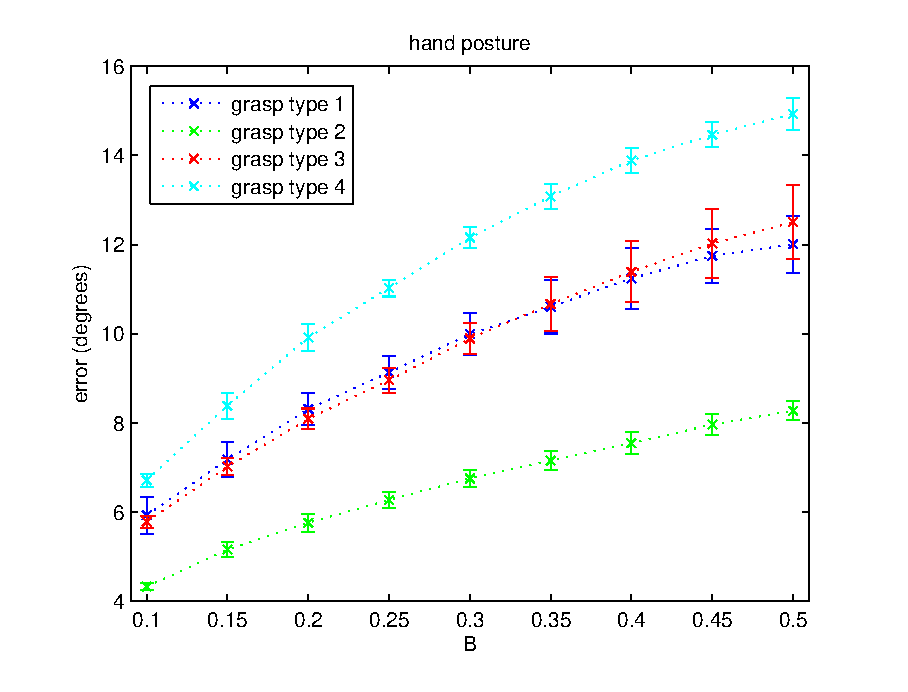
\includegraphics[width=0.45\textwidth]{error_pst_cluster.eps} &
      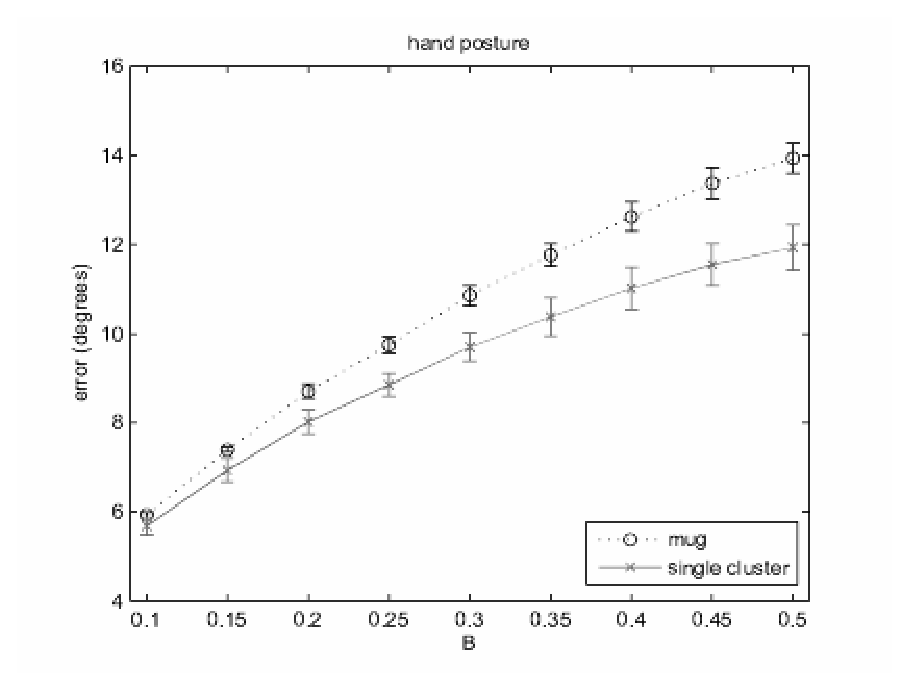
\includegraphics[width=0.45\textwidth]{error_pst_cmp_cluster.eps} \\
      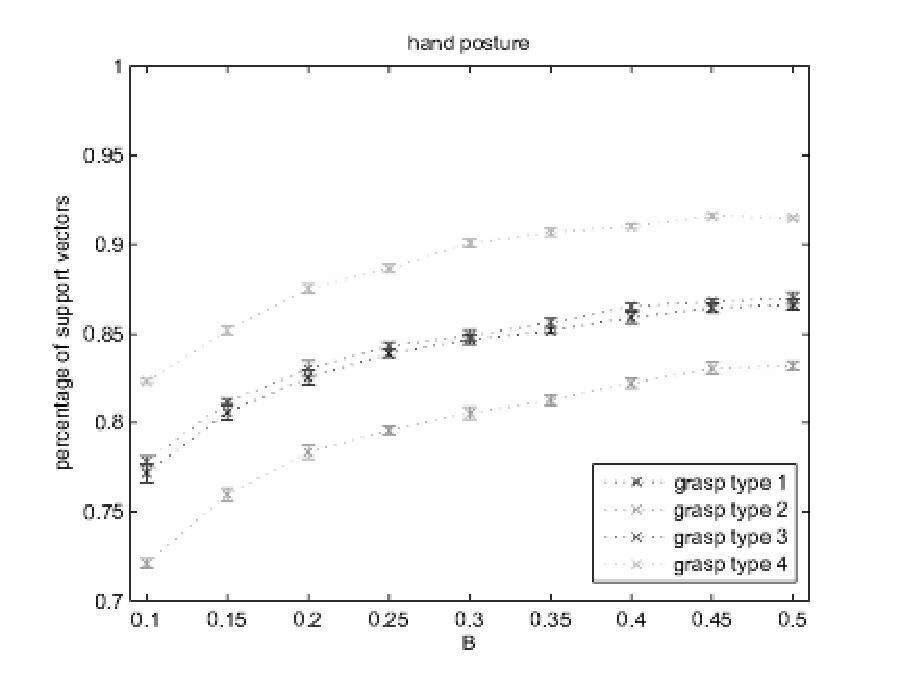
\includegraphics[width=0.45\textwidth]{error_pst_SV_cluster.eps} &
      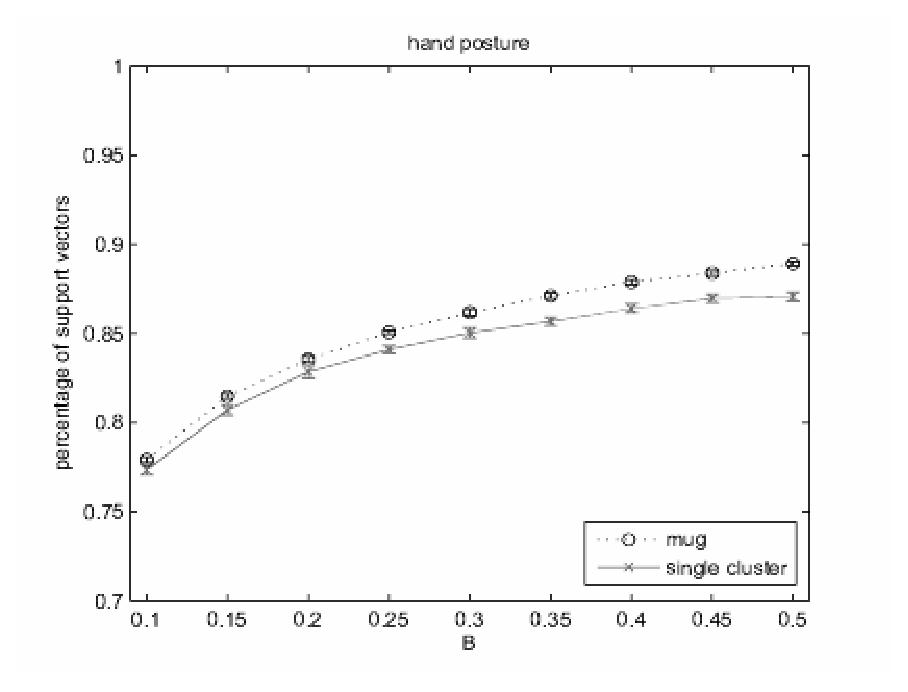
\includegraphics[width=0.45\textwidth]{error_pst_cmp_SV_cluster.eps} \\
    \end{tabular}
    \caption{Comparison among regression on single grasp types (left
      column) and between regression with/without knowledge of the grasp
      type (right column).}
    \label{fig:clustering}
  \end{center}
\end{figure}

First of all, it must be noticed (left column) that there is a
considerably different error among the types of grasps, type $4$ begin
the more complex, followed by $1$ and $3$ having the same complexity,
and $2$ being the easiest one. This ranking is confirmed by the
percentage of SVs graph (bottom left). But, as well, the error on the
single grasps is \emph{smaller} than that on the mug (green curve in
Figure \ref{fig:err_all}, bottom left graph) in three cases out of
four, and only slightly larger in the case of grasp type $4$. This
suggests that the machine is able to learn well a number of different
grasp types, without ``specialising'' on one easy type.

Secondly, consider the right column of the Figure. We have made an
analogous comparison as that shown in Figure \ref{fig:err_all}, right
column: in that case we compared the errors obtained with and without
prior knowledge of the object to be grasped; here we compare the
errors \emph{on the mug}, with and without prior knowledge of the type
of grasp. The result is that knowing in advance the type of grasp
makes the machine even more accurate and smaller than it used to be
before.


\section{DISCUSSION}
\label{sec:Conclusions}
With this initial experiment we really pose further questions and
sketch future research rather than draw definite conclusions. The
machine learning questions addressed in this paper do indeed have an
answer, albeit partial; on the other hand, it remains difficult to say
something other than speculations when comparing these results to
neuroscience.

In short, the answer to the two questions posed in Section
\ref{sec:exp_desc} is that we can predict well given that we have
access to motor information at least during learning, and that knowing
the objects to be grasped improves the ability to predict the outcome
of an action. There are many caveats in this experiment, as for
example, the question on whether a pre-processing of the data through
clustering could improve performance further: i.e., given that objects
afford certain grasping postures and they are executed with high
probability. In humans the quality of the prediction of grasping is a
function of the expectancies of the various possible grasp types which
are in turn determined by the past experience of manipulation of the
target object\footnote{personal communication with Luciano Fadiga.}.

The solution found by the SVMs detailed in the previous Section is
optimal, since the dependence from hyperparameters has been optimized
out in our case by grid search and cross-validation that although
expensive is known to provide good results. An analysis of the
solution should thus provide an accurate characterization of the
problem qua the data set that has been collected.

In this sense (and only in this sense) we have shown that by
partitioning the training set per object provides a general
improvement of the quality of the solution and simultaneously of the
training time (worst case $O(l^3)$ versus $O(3 \cdot (l/3)^3)$ in our
case with $3$ objects and $l$ the total number of samples). This can
be an effective strategy when the world affords such an intuitive
partitioning as for objects (seen as discrete entities).

This is also true from what is known about the brain structures that
control grasping where the presence of a target object, its shape and
affordance, and in general any contextual cue, are coded separately by
different populations of neurons and influence simultaneously the
response of the neurons that enact specific motor plans. After motor
prediction is in place, the next step, that of recognizing the action
of another individual is conceptually simple since it amounts to
building a classifier on highly predictable motor trajectories.

Another interesting question that is left to future research is
whether we can investigate the complexity of the controllers of
reaching and grasping (which are known to develop separately in
humans) from the complexity of the learned models or as a
consequence of the prediction error.

Clearly, the fact that we can train such models is prone to
be applied in various contexts, as we mentioned, ranging from control
of robots through interpretation and prediction of human behavior in
particular for man-machine communication.


{\small
\bibliographystyle{alpha}
\bibliography{paper}
}

\end{document}
